\clearpage
\setcounter{page}{1}
\maketitlesupplementary
\def\phiorg{\mathop{\phi_{\rm{Org}}}\nolimits}

\section{Benchmarking existing DL detectors}
\label{sec:benchmarking}
\begin{figure}[!t]
    \centering
    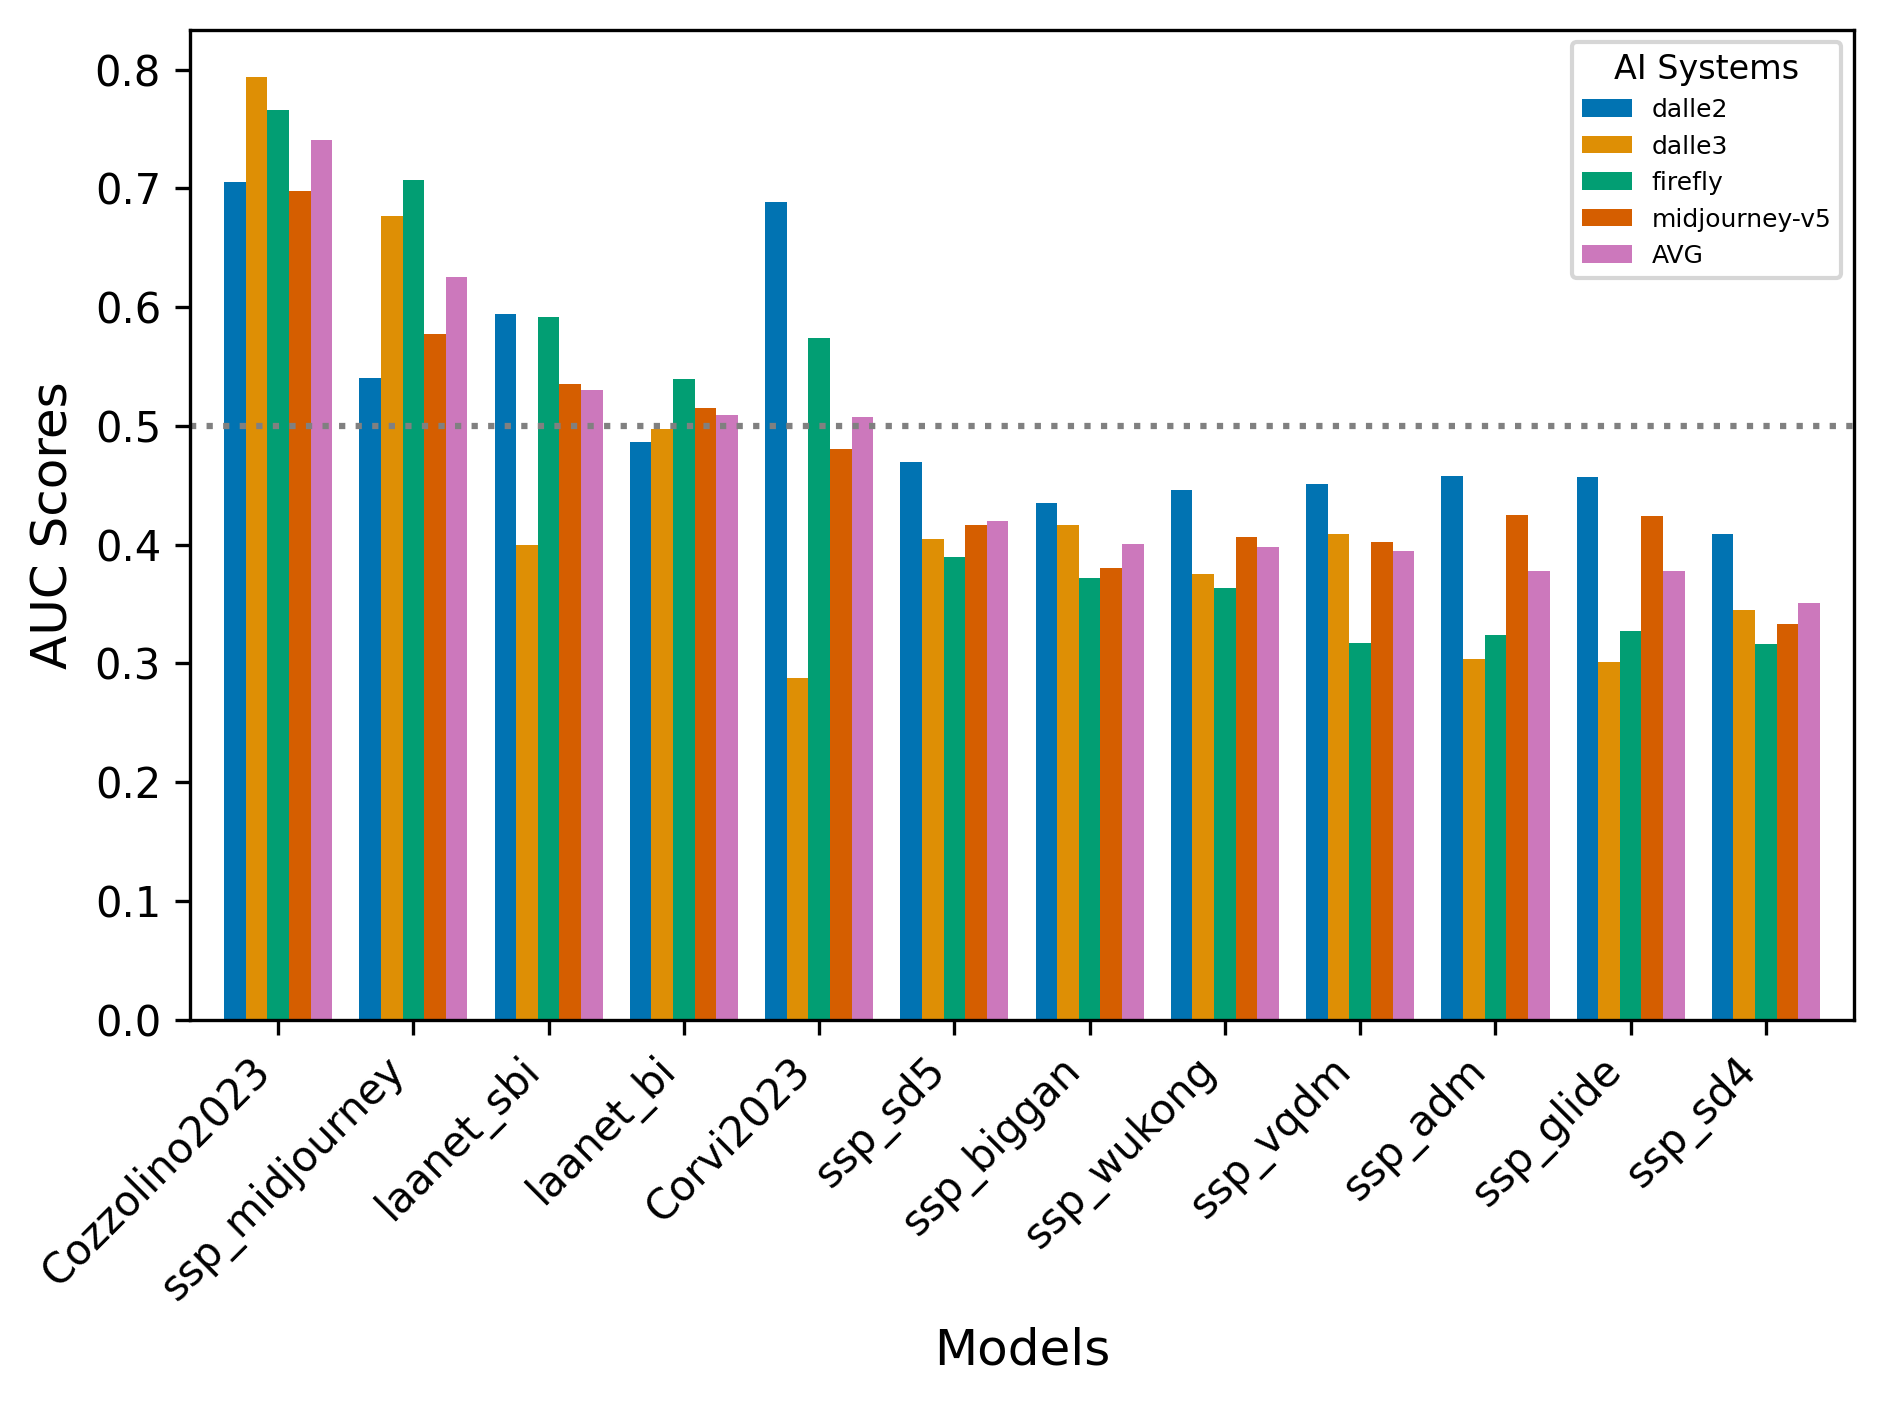
\includegraphics[width=0.95\linewidth]{images/auc_bench.png}
    \caption{Area Under ROC curve for various models on postprocessed images. Arranged in descending order of average AUC.}
    \label{fig:auc_bench}
\end{figure}
\red{
Existing litreature contains various methods for detecting AI generated images using machine learning models. These methods can be classified primarily into a) Artifact based methods and b) VLM based methods. Artifact based methods \citep{wang2020cnn,gragnaniello2021gan,mandelli2022detecting,chai2020makes,nguyen2024laa} leverage fingerprints of image generators or noise patterns of camera \citep{chen2024single} to detect AI generated image. While this method is effective, it often does not generalize well to unseen generators and artifacts are often lost under operations like JPEG compression, resizing and random crop. VLM based methods \citep{ojha2023towards,cozzolino2024raising} leverage the join image-language feature space to detect fake images.

In this era of social media and freely available text-to-image generators the task of detection AI generated images has gained a lot of attention. A lot of different approaches are available but we found a lack of common benchmark. A lot of authors often do not report results on realistic scenarios like highly compressed images. \citet{cozzolino2024raising} benchmark state-of-the-art detectors and show through extensive experiments that VLM based method perform well on postprocessed images while performance of artifact based methods often fall to near random chance. Despite this effort there still existed new detectors \citep{nguyen2024laa,chen2024single} that were not benchmarked under the same condition. We benchmark all detectors on the dataset and under transformations described in \Cref{subsec:exp_dl}. The Area Under Curve and Accuracy for the models not benchmarked in \citep{cozzolino2024raising} are visualized in \Cref{fig:auc_bench} and \Cref{fig:acc_bench} respectively. Our benchmarking reinforced the findings of \citet{cozzolino2024raising} and shows the superiority of VLM based detectors. Hence, we choose to leverage VLM based detector in our framework.
}

\begin{figure}[!t]
    \centering
    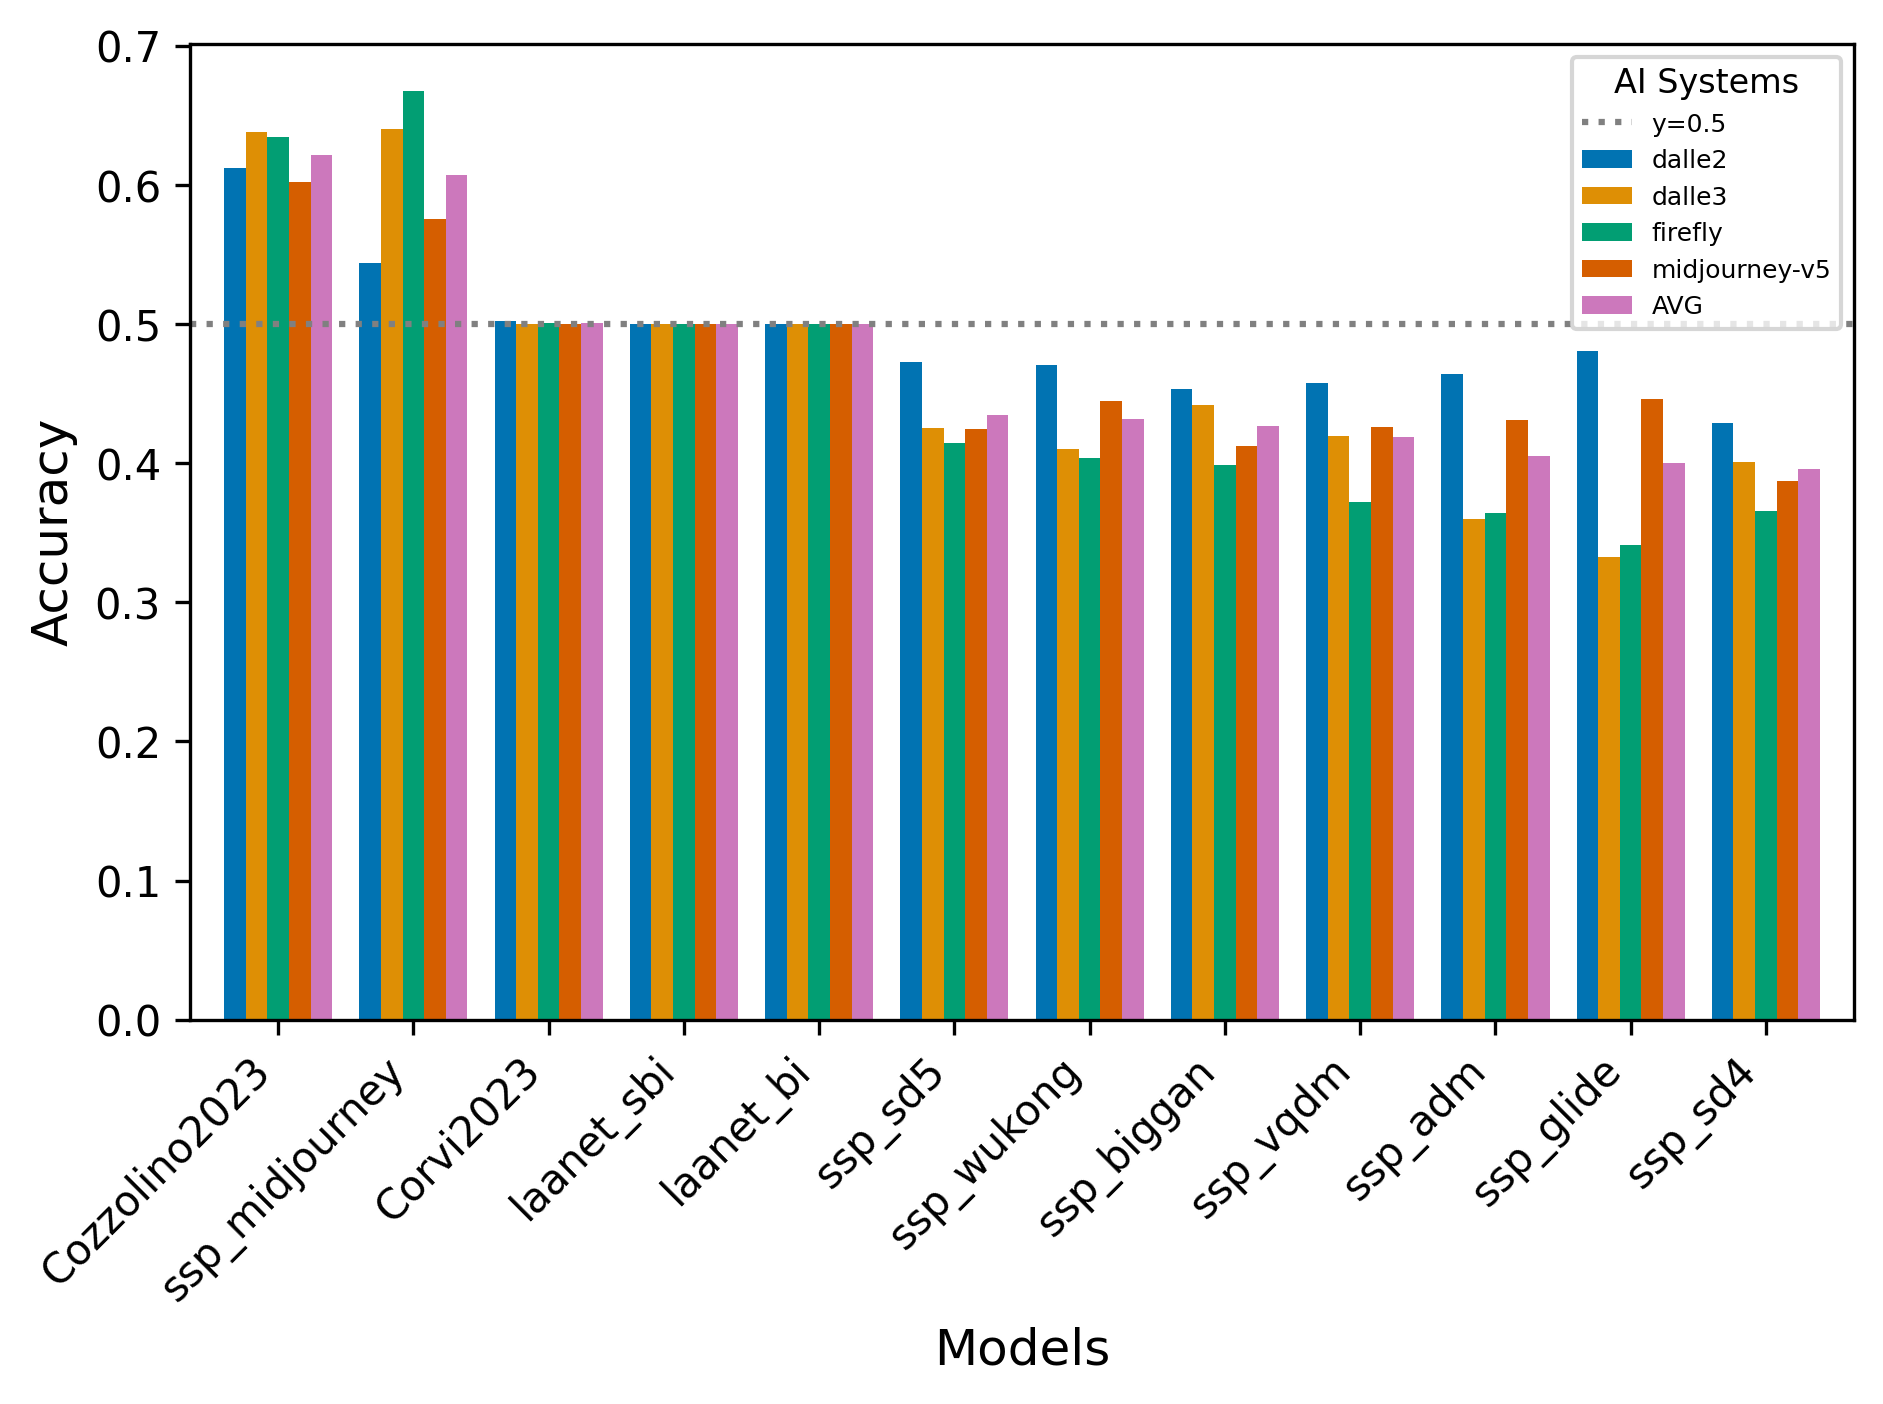
\includegraphics[width=0.95\linewidth]{images/acc_bench.png}
    \caption{Accuracy for various models on postprocessed images. Arranged in descending order of average accuracy.}
    \label{fig:acc_bench}
\end{figure}
\section{Ablation Study}
\label{sec:ablation}
\begin{table*}[h]
    \centering
    \small
    \begin{tabular}{lccccccccc}
        \toprule
        VLM & Backbone&Resolution & Classifier & Text & DALL·E 2 & DALL·E 3 & Firefly & Midjourney v5 & Avg \\
        \midrule 
        CLIP & ViT-L & 224& Zero-shot & Fixed & 0.524&0.558&0.550&0.534&0.542 \\
        CLIP & ViT-L & 224& Zero-shot & BLIP & 0.508&0.476&0.475&0.474& 0.483 \\
        DFN & ViT-H & 224& Zero-shot & BLIP &0.609&0.818&0.670&0.663 & 0.690 \\
        CLIP & ViT-L & 224 & SVM & - &  0.680&0.74&0.646&0.627&0.673 \\
        DFN & ViT-H & 224& SVM & - & \textbf{0.792} & \textbf{0.997} & \textbf{0.921} & \textbf{0.934} & \textbf{0.911} \\
        SigLIP & so-ViT-400M & 224& SVM & - & 0.663 & 0.996 & 0.896 & 0.909 & 0.866 \\
        \bottomrule
    \end{tabular}
    \caption{Ablation study on AI detection model architecture with individual model performance. Table contains accuracy values on non postprocessed images.}
    \label{tab:ablation_expanded}
\end{table*}
\red{
\Cref{sec:benchmarking} clearly motivates the use of VLMs for generalizable and robust detector. Choice of architecture and exact method of detection can significantly affect detection. We have to choose which VLM to use, size of backbone (B/L/H) to use and the method of detection.  We can either use zero shot capablities of VLMs or train a classifier on top of features extracted from VLMs. If we choose zero shot methods we could either use fixed text template or generate custom text using state of the art models like BLIP.
We explain each choice in detail below.

\subsection{Choice of Backbone}
\citet{radford2021learning} introduced contrastive learning of joint language image embedding space. The pioneering CLIP model was adopted and used extensively due to its generalization and few shot capabilities. Follow-up work \citep{fang2023data,zhai2023sigmoid} improved this through various strategies, including additional loss terms, a new dataset created using novel data filtering strategies and changes in normalization. Open CLIP \citep{ilharco_openclip_2021} has trained a range of these models on varying backbones, datasets and resolutions. We find that DFN \citep{fang2023data} and SigLIP-based models \citep{zhai2023sigmoid} have the highest zero-shot imagenet accuracies. Our task involves using these models for downstream tasks, so we use zero-shot ImageNet accuracies to indicate which model could perform well on our task. Thus, we experiment with DFN and SigLIP-based models along with Open AI's CLIP. We have three different backbones, i.e. ViT-L, ViT-H and so-ViT-400M. Results are detailes in \Cref{tab:ablation_expanded}. We observe that the DFN-based ViT-H backbone outperforms the CLIP-based ViT-L backbone and SigLIP-based so-ViT-400M backbone when using the same classification strategy, i.e. SVM. It also outperforms CLIP-based ViT-L when we do zero-shot classification. So, the DFN-based ViT-H backbone is the clear choice for our detection model. We note that the SigLIP-based so-ViT-400M backbone has performance comparable performance, so we include it in further experiments.


\subsection{Method of Detection}
\citet{cozzolino2024raising} tested Support Vector Machine, Logistic Regression (LR), Mahalanobis distance (MAH), Gaussian Naive Bayes classifier
(GNB), Soft voting k-Nearest Neighbor (SNN) with Open AI's CLIP and found out that SVM performs the best on the task of detection AI generated images. However, CLIP's zero shot capablities were not tested. So we test three classification strategies, namely zero-shot classification with fixed text template, zero-shot classification with BLIP generated text template and SVM. \Cref{tab:ablation_expanded} clearly shows SVM performs better, so we use SVM in our final detector.
}


\red{
\section{Adversarial Training}\label{sec:adversarial}

In this section we discuss the adversarial fine-tuning implementation details for DinoHash and DL based detector.


\subsection{DinoHash}
Given a hashing model, $H$, we would like to finetune it such that an adversarial perturbed image, $x'$, produces the same hash as the original image, $x$ where $\norm{x-x'}_\infty \leq \epsilon$, i.e. we would like that $H(x') \approx H(x)$. Hence, we initially formulated the following objective for finetuning:

\begin{align}
H_{robust}=&\argmin_{H}\sum_{i=1}^n \max_{\norm{x_i'-x_i}_\infty \leq \epsilon} \norm{H(x_i')-H(x_i)}_1.
\end{align}

The downside of this approach was that it led to a collapse of the hashing function and caused it to produce the same hash for all images, which is undesirable. This behaviour can be explained since the proposed loss function is perfectly minimized.

This led us to formulate our second optimization problem

\begin{align}
H_{robust}=&\argmin_{H}\sum_{i=1}^n \max_{\norm{x_i'-x_i}_\infty \leq \epsilon} \norm{H(x_i')-H_{orig}(x_i)}_1.
\end{align}

Where $H_{orig}$ denotes the original, non-robust hashing model. This ensured that the model retains its original hashing capability. The inner maximization problem was solved by adapting APGD \citenum{autoattack}, a popular algorithm for adversarial attacks, to our use case.

Since the heaviside step function is non-differentiable, we used cross-entropy loss on the logits before the binarization step. Furthermore, we observed that adding a clean-loss term aided the optimization process and resulted in faster convergence. The final loss function used in code was:

\begin{equation}
\begin{split}
L(x_i)= \text{CE}(\hat{H}(A(x_i)), \: \hat{H}_{orig}(x_i)) \: + \\
\alpha \cdot \text{CE}(\hat{H}(x_i), \: \hat{H}_{orig}(x_i))
\end{split}
\end{equation}


Here $A(x)$ represents the attacked version of image $x$ generated by APGD with $\epsilon=8/255$, CE represents the cross-entropy loss with the second term as the target logit, $\hat{H}$ represents the deep hashing model without the binarization step, and $\alpha$ represents the loss weightage for clean examples and was set to $500$ in our experiments. 
\begin{table*}[htbp]
    \centering
    \begin{tabular}{l c c c c c c}
        \toprule
       ` & \multicolumn{2}{c}{Clean Data} & \multicolumn{2}{c}{Adversarial} & \multicolumn{2}{c}{Adversarial} \\
        \cmidrule(lr){2-3} \cmidrule(lr){4-5} \cmidrule(lr){6-7}
        $\boldsymbol{\varepsilon}$
 & \multicolumn{2}{c}{-} & \multicolumn{2}{c}{4} & \multicolumn{2}{c}{8} \\
        \midrule
        & Non-Robust & Robust & Non-Robust & Robust & Non-Robust & Robust \\
        \midrule
        DALL·E 2 & 0.559 & 0.54 & 0.645 & 0.838 & 0.662 & 0.822 \\
        DALL·E 3 & 0.972 & 0.847 & 0.66 & 0.867 & 0.685 & 0.864 \\
        Firefly & 0.623 & 0.574 & 0.632 & 0.826 & 0.641 & 0.825 \\
        Midjourney v5 & 0.689 & 0.614 & 0.651 & 0.85 & 0.662 & 0.838 \\
        Average & 0.711 & 0.644 & 0.647 & 0.845 & 0.663 & 0.837 \\
        \bottomrule
    \end{tabular}
    \caption{Comparison of Non-Robust and Robust Models Across Attack Types and Generators}
    \label{tab:robust_dldetector}
\end{table*}
We fine-tune DinoHash on DiffusionDB using the loss function defined above for $20,000$ steps with a batch size of $256$ using the AdamW optimizer. The adversarial examples were generated using APGD with $10$ steps.

We compare the adversarial robustness of DinoHash against different baseline models in \autoref{tab:adv_hash}. We note that for all baseline models, the adversarial attack achieves near-perfect accuracy, significantly underscoring the insecurity of their application as compared to DinoHash. 

We would like to mention that we were initially experimenting with DISCO \citenum{disco} to enhance robustness against adversarial attacks. However, our experiments indicated that DISCO is extremely vulnerable to standard PGD attacks, despite prior claims that the Backward Pass Differentiable Approximation Attack \citenum{obfuscated} was the strongest. This suggests that its reported robustness is heavily overstated.

\renewcommand{\arraystretch}{1.5}
\begin{table}[h]
    \centering
    \begin{tabular}{cccc}
        \toprule
        $\epsilon$ & DinoHash & NeuralHash & Stable Signature \\
        \midrule
        $\frac{4}{255}$ & $\textbf{62.0\%}$ & $0.1\%$ & $0.0\%$ \\
        $\frac{8}{255}$ & $\textbf{64.8\%}$ & $0.0\%$ & $0.0\%$ \\
        \bottomrule
    \end{tabular}
    \caption{Performance of different models under adversarial perturbations with the APGD attack performed using $100$ steps}
    \label{tab:adv_hash}
\end{table}

}


\subsection{DL based detector}

\red{
\citet{schlarmann2024robust} proposed an unsupervised method to adversarially finetune CLIP that preserves performance on downstream tasks. We use this method for adversarial finetuning of our model. We first discuss the method below. Then we discuss our results.

\textbf{Method} We aim to minimize the distance between the embeddings of unattacked images for original CLIP model and corresponding adversarially attacked image for the robust model. The idea is that if embeddings are unaffacted by attack then performance on downstream task will be preserved. In the following we denote with $\phiorg$ the original CLIP encoder which is frozen. $\phi(z)$ is the encoder that is being trained. x is the input image and z is the corresponding adversarially attacked image. We propose the following embedding loss:

\begin{align}\label{eq:fare}
L_{\textrm{\ours}}(\phi,x)=&\,\max_{\norm{z-x}_\infty \leq \epsilon} \norm{\phi(z)-\phiorg(x)}^2_2.
\end{align}

\textbf{Training Details} We use PGD attack for training with $\epsilon$ 4 and $l_\infty$ norm. We use 10 iterations of attack per image with batch size of 128. We train for 20000 iterations on ImageNet dataset. We use ADAM optimizer with a learning rate of 1e-5, weight decay of 1e-4 and learning rate warmup of 1400 steps. We use L2 loss for attack. The training parameters are consistent with \citep{schlarmann2024robust}.

\textbf{Results} We do adversarial evaluation for just the finetuned version of our detector with DFN ViT-H backbone and 224 resolution. We evaluate using 100 iterations of APGD attack with binary cross entropy loss. We evaluate non-robust and adversarially finetuned model on clean data, attacked data with epsilon 4 and attacked data with epsilon 8. We present the results in \Cref{tab:robust_dldetector}. We observe that the adversarially trained model's performance does not degrade much on clean data but it performs much better on attacked data.

}

\red{
\section{Securing User Data without FHE}\label{sec:apx-mpc}

Figure~\ref{fig:protocol} presents an overview of our second proposal, comprising the following key steps:

\begin{figure}[t]
  \centering
  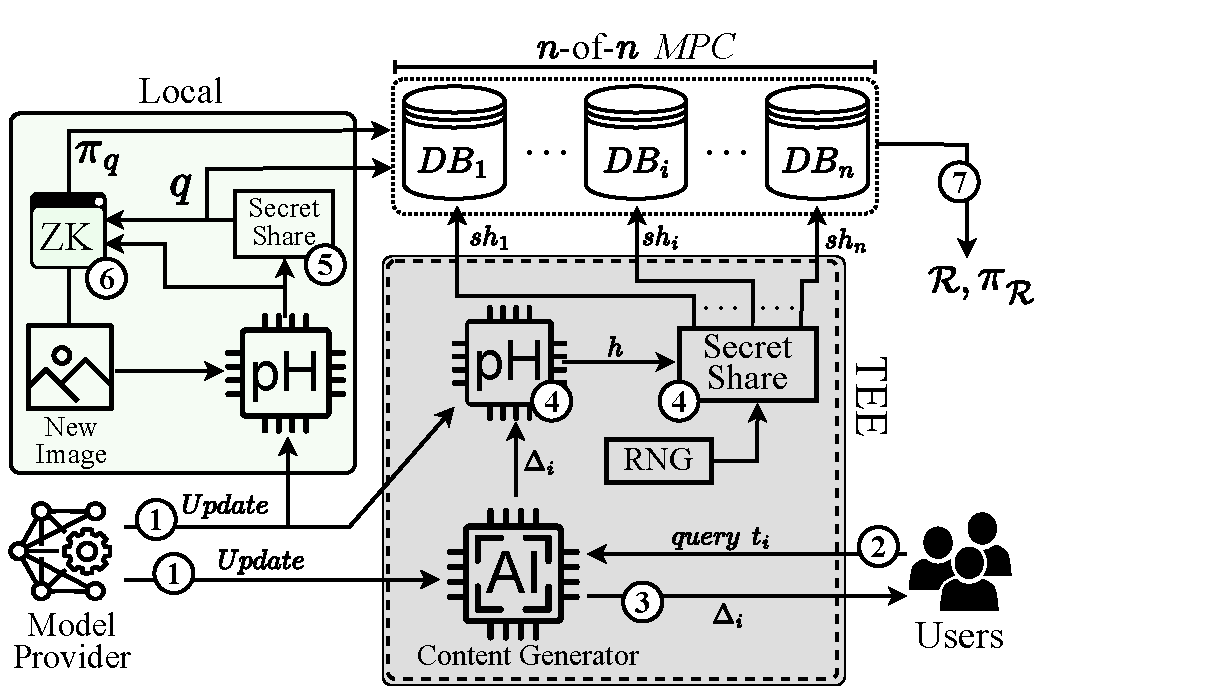
\includegraphics[width=\linewidth,trim={0 0 3.2cm 0},clip]{figures/protocol_v3.pdf}
   \caption{High level overview of the protocol.}
   \label{fig:protocol}
\end{figure}

\begin{itemize}
    \item[] \circled{1} The \textit{model provider} is responsible for fine-tuning and updating the generative model~(e.g., OpenAI) with write-only access to the TEE. This ensures that the \textit{model provider} cannot eavesdrop on user queries. Additionally, the \textit{model provider} can update the perceptual hash function as needed.\\

    \item[] \circled{2}, \circled{3} The user $u_i$ submits a prompt to the server and receives the generated image as the result.\\
    
    \item[] \circled{4} The TEE calculates the pHash of the resulting image $\Delta_i$ and distributes the shared pHash components~($sh_1,\dots, sh_n$) among $n$ parties~($DB_1,\dots,DB_n$). During this phase, neither the generated image nor its related information is stored. No single party can retrieve any information about the image without collaboration from the others.\\
    
    \item[] \circled{5} When a new image is checked against the shared database, its pHash is first calculated, and then this value is distributed among the $n$ parties.\\
    
    \item[] \circled{6} The proof of ownership for the original image is calculated and sent to the databases alongside the shared pHash value. Given the input size of the pHash model is $224 \times 224$, the owner of the query image $x$ proves knowledge of a larger image $X$ that has been resized to $224 \times 224$. The user also demonstrates that the resized image $x$ has a pHash value of $q$, which is shared as $[q]=\{q_1,\dots,q_n\}$. Moreover, since no party will ever gain access to all of these shares~($q_1,\dots,q_n$), it is necessary to prove to each party that they posses a unique and correct share of of $[q]$. To this end, we propose building a Merkle tree $\Delta$ out of these shares and prove each party is given a certain unique leaf of $\Delta$. Finally, to connect these claims, commitments for both the original and resized versions of the image are needed, for which we employ collision-resistant image hashing techniques from prior work~\cite{vimz, veritas}. More precisely, the user asserts the following statement:
    \begin{equation}\label{eq:state-image}
        \begin{split}
        \hspace{-0.5cm}S\bigr[\mathcal{R}_\Delta, \underline{[q], i}, h_X, h_x \bigr] \: :\: \bigr\{ \exists \: X,  x\:\:\: s.t. \:\:\: x{=}f{\downarrow}(X) \\
         \mbox{ and }  h_X=\mathcal{H}_\mathcal{C}(X) \mbox{ and } h_x= \mathcal{H}_\mathcal{C}(x) \\
        \mbox{ and } q=\mathcal{H}_\mathcal{P}(x) \mbox{  and  } \exists\:\mathcal{O}(\mathcal{R}_\Delta, q_i, i\bigr)\}
        \end{split}
        % \raisetag{20.5pt}
    \end{equation}
    We note that the prover generates $n$ distinct proofs for $i \in \{1, \dots, n\}$ to ensure each party has received a unique share of $[q]$.\\
    
    \item[] \circled{7} The parties in the MPC-based database verify their received proofs and execute the query for the shared pHash value $[q]$. They then participate in the MPC to execute the given query on the shared DB. Based on the query result, the parties engage in a collaborative zkSNARK protocol to achieve public auditability, as follows:
    \begin{itemize}
        \item \textbf{Match:} If there is a match, the result of the execution includes the index of the matched values. Therefore, the parties claim the following statement:
        \begin{equation}\label{eq:state-match}
            \begin{split}
            \hspace{-0.5cm}S\bigr[\mathcal{R}_\Delta, [q] ,t\bigr] \: :\: \bigr\{ \exists \: id\in \mathbb{N}\:\:\: s.t. \:\:\: \gamma=\prod_0^n \mathit{DB}_i[id]\\
            \hspace{-0.5cm}\mbox{ and } \mathcal{R}_\Delta=\mbox{\texttt{Merkle\_Root}}(\cup \: q_i)\mbox{ and }  \mbox{\texttt{HD}}(q,\gamma) {\leq} t\bigr\}
            \end{split}
            % \raisetag{20.5pt}
        \end{equation}
        \item \textbf{No Match:} If there are no matches found in the database, then parties will claim following statement:
        \begin{equation}\label{eq:state-no-match}
            \begin{split}
            \hspace{-0.5cm}S\bigr[\mathcal{R}_\Delta, [q] ,t\bigr] \: :\: \bigr\{ \forall \: id\in \mathbb{N}_{\{DB\}}\: \bigr|\: \gamma=\prod_0^n \mathit{DB}_i[id]\\
            \hspace{-0.5cm}\mbox{ and } \mathcal{R}_\Delta=\mbox{\texttt{Merkle\_Root}}(\cup \: q_i)\mbox{ and } \mbox{\texttt{HD}}(q,\gamma) {>} t \bigr\}
            \end{split}
            % \raisetag{20.5pt}
        \end{equation}
    \end{itemize}
    It should be noted that while proving the statement in equation~\ref{eq:state-match} is relatively feasible, the statement in equation~\ref{eq:state-no-match} is computationally expensive. However, we argue that in most scenarios, the most critical supporting proof would be the case where a match is found, as expressed in equation~\ref{eq:state-match}.

\end{itemize}


}